\chapter{Bunyi: Penghasilan dan Perambatan}\label{ch:g7:sound-production}

Kamu sudah tahu sejak masa kecil bahwa \omterm{def:g3:sound-around-us:sound}{bunyi} lahir di dalam sebuah
\omterm{def:g3:sound-around-us:vibration}{getaran} lalu mati di dalam kehampaan --- butiran berasnya menari,
belnya di dalam toples terdiam. Yang belum kamu punyai adalah nama
pengantar pesannya. Kini kamu memiliki dunia \omterm{def:g7:states-of-matter:molecule}{molekul}, dan seluruh
perjalanan \omterm{def:g3:sound-around-us:sound}{bunyi} --- dari sehelai dawai gitar sampai ke gendang
telingamu, menembus \omterm{def:g2:air-around-us:air}{udara}, air, atau baja --- akhirnya dapat ditonton
dari dalam.

\section{Para pengantar pesan}

\begin{definition}[Medium]\label{def:g7:sound-production:medium}
\emph{Medium}\index{medium} (bentuk jamaknya \emph{media}) adalah zat
yang dilewati \omterm{def:g3:sound-around-us:sound}{bunyi} ketika berjalan: \omterm{def:g2:air-around-us:air}{udara}, air, kayu, baja --- wujud
mana pun sanggup melayani, karena semuanya kerumunan \omterm{def:g7:states-of-matter:molecule}{molekul}. Yang
tidak dapat diseberangi \omterm{def:g3:sound-around-us:sound}{bunyi} mana pun adalah ketiadaan kerumunan:
hampa \omterm{def:g2:air-around-us:air}{udara}, panggung yang kosong.
\end{definition}

\begin{proposition}[Bagaimana bunyi berjalan]\label{prop:g7:sound-production:travel}
Sumber yang bergetar mendorong \omterm{def:g7:states-of-matter:molecule}{molekul} di sampingnya; \omterm{def:g7:states-of-matter:molecule}{molekul} itu
berdesak pada tetangganya lalu memantul; tetangganya mendorong barisan
berikutnya pada gilirannya. Dorongannya --- perasan kerumunan yang
berjalan --- melesat ke luar dari sumbernya ke segala arah, \omterm{def:g7:states-of-matter:molecule}{molekul}
mengestafetkan \omterm{def:g7:states-of-matter:molecule}{molekul}, walaupun tiap \omterm{def:g7:states-of-matter:molecule}{molekul} sendiri hanya bergoyang
di sekitar tempatnya. \omterm{def:g3:sound-around-us:sound}{Bunyi} adalah \emph{estafetnya}, bukan
pelarinya: pesannya berjalan; para pengantar pesannya tinggal di rumah.
\end{proposition}

\begin{omfigure}
\begin{tikzpicture}[scale=0.85]
  \draw[thick] (0.2,0.4) -- (0.2,2.2);
  \draw[thick] (0.5,0.4) -- (0.5,2.2);
  \node[above, font=\small] at (0.35,2.3) {pelat yang bergetar};
  \foreach \x in {1.0,1.25,1.5,2.4,3.3,4.2,4.45,4.7,5.6,6.5,
      7.4,7.65,7.9,8.8,9.7} {
    \fill[omDef] (\x,1.3) circle (0.11);
  }
  \draw[-Stealth, very thick, omThm] (1.0,2.0) -- (2.6,2.0);
  \node[above, font=\small, omThm] at (1.8,2.1)
    {perasannya berjalan};
  \node[below, font=\small] at (1.3,0.8) {berdesak};
  \node[below, font=\small] at (3.3,0.8) {merenggang};
  \node[below, font=\small] at (4.6,0.8) {berdesak};
  \node[below, font=\small] at (6.5,0.8) {merenggang};
  \node[below, font=\small] at (7.8,0.8) {berdesak};
\end{tikzpicture}

{\small \omterm{def:g3:sound-around-us:sound}{Bunyi} di dalam \omterm{def:g2:air-around-us:air}{udara}: dorongan sumbernya berjalan sebagai
estafet perasan menembus kerumunan \omterm{def:g7:states-of-matter:molecule}{molekulnya} --- tiap \omterm{def:g7:states-of-matter:molecule}{molekul}
bergoyang di tempatnya, polanya yang melesat terus.}
\end{omfigure}

\begin{example}[Toplesnya, akhirnya terjelaskan]\label{ex:g7:sound-production:jar}
Bel yang termasyhur dibungkam itu kini mengakui mekanismenya. Memompa
keluar \omterm{def:g2:air-around-us:air}{udaranya} menyingkirkan kerumunannya: dinding bel yang bergetar
mendorong ketiadaan, tidak terbentuk estafet, dan tidak ada pesan yang
menyeberangi kacanya. Belnya tidak pernah berhenti --- ia kehilangan
para pengantar pesannya. Dan kesunyian besar antariksa langsung
menyusul: di antara \omterm{def:g4:solar-system:star}{bintang} tidak ada kerumunan yang membawa jeritan.
\end{example}

\begin{example}[Nyaring, lirih, dan kehabisan tenaga]\label{ex:g7:sound-production:loud}
Dorongan yang lebih keras membuat perasan yang lebih kuat: \omterm{def:g3:sound-around-us:sound}{bunyi} yang
lebih nyaring. Dan selagi estafetnya menyebar --- riak kolam dalam
tiga dimensi --- tiap perasannya dibagikan atas kulit kerumunan yang
kian luas dan kian luas, sehingga melemah menurut jarak: itulah
sebabnya teriakan memudar, dan mengapa musik tetangga hanya gumam
menembus dua tembok. Tidak satu pun dari hal ini memerlukan hukum
baru: fisika kerumunanlah yang membayar segalanya.
\end{example}

\begin{omfigure}
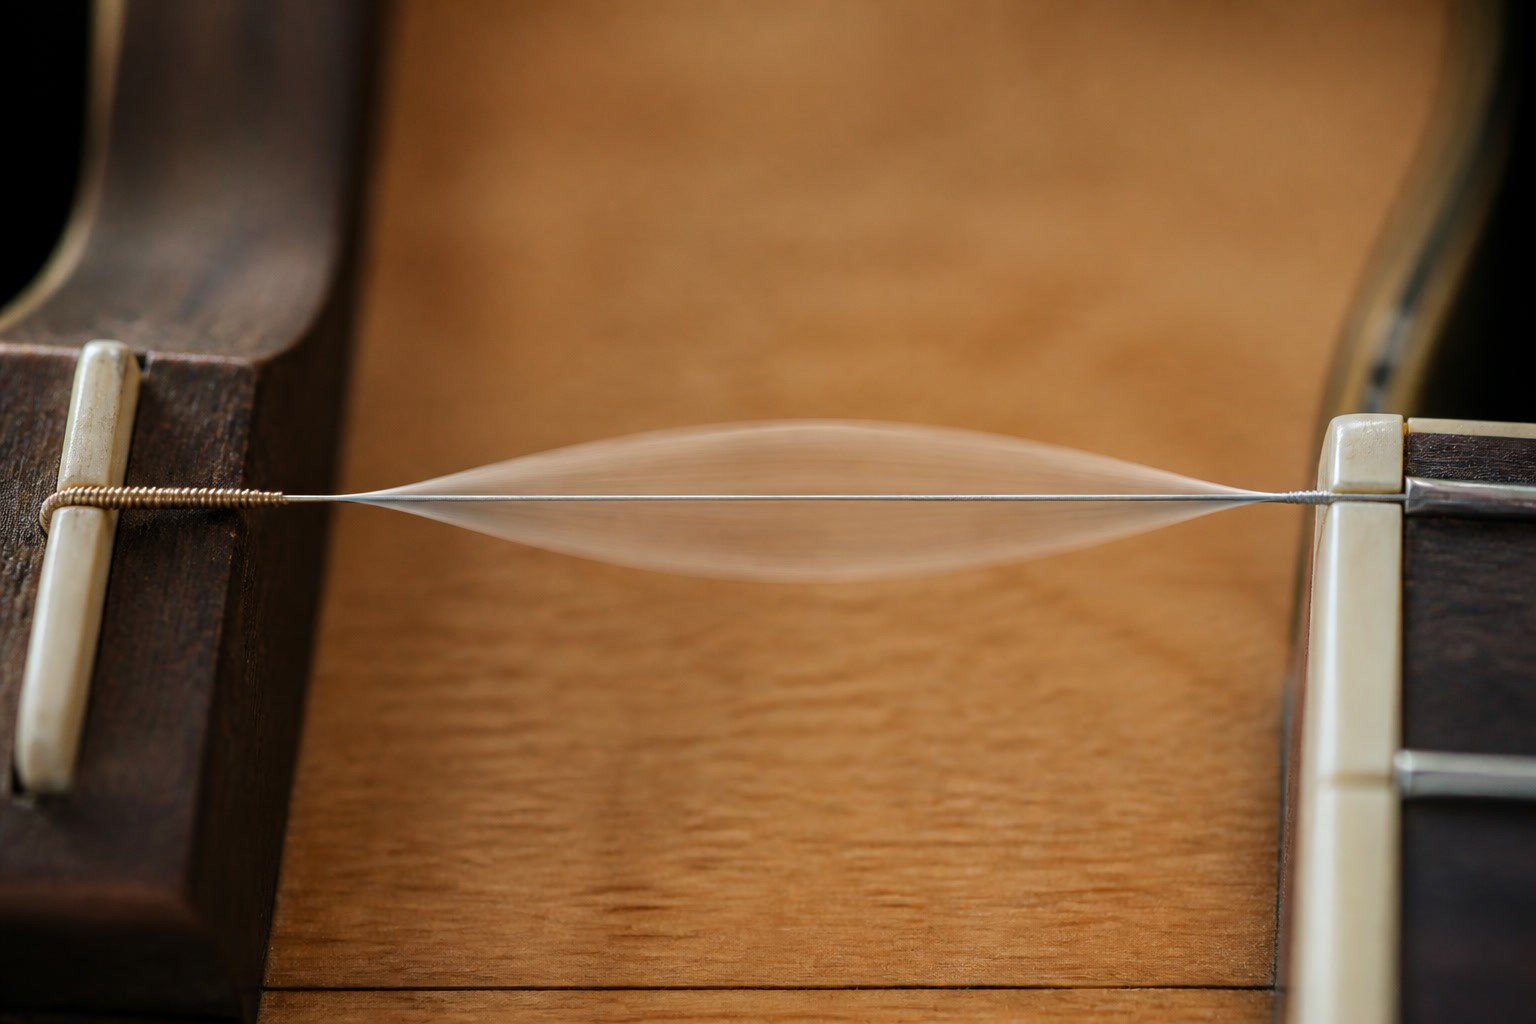
\includegraphics[width=0.55\linewidth]{images/book1/ai/g7-sound-string-blur.jpg}

{\small Sehelai dawai yang dipetik, dipotret di tengah lagunya: \omterm{def:g3:sound-around-us:vibration}{getarannya} mengaburkannya menjadi pita yang lebar, paling lebar di tengah, dan diam pada kedua ujungnya yang terpancang.}
\end{omfigure}

\section{Tiap medium mempunyai langkahnya}

\begin{proposition}[Kelajuan bunyi bergantung pada mediumnya]\label{prop:g7:sound-production:speeds}
\omterm{def:g7:motion-average-speed:formula}{Kelajuan} estafetnya adalah sifat kerumunannya:
\begin{enumerate}
  \item di dalam \omterm{def:g2:air-around-us:air}{udara}: kira-kira \qty{340}{m/s};
  \item di dalam air: kira-kira \qty{1500}{m/s} --- empat kali lebih
        cepat;
  \item di dalam baja: kira-kira \qty{5000}{m/s} --- lima belas kali
        lebih cepat daripada \omterm{def:g2:air-around-us:air}{udara}.
\end{enumerate}
Polanya: makin rapat \omterm{def:g7:states-of-matter:molecule}{molekul} sebuah \omterm{def:g7:sound-production:medium}{medium} bersentuhan, makin cepat
mereka mengoperkan dorongannya. \omterm{def:g7:states-of-matter:molecule}{Molekul} \omterm{def:g2:air-around-us:air}{udara} yang beterbangan harus
menyeberangi celah lebih dahulu untuk mengantar; kerumunan air yang
bersentuhan mengestafet dengan sigap; barisan baja yang terkunci
mengoper pesannya hampir dari tangan ke tangan.
\end{proposition}

\begin{omfigure}
\begin{tikzpicture}
\begin{axis}[omaxis, width=10.4cm, height=4.6cm, xbar,
    xlabel={kelajuan bunyi (\unit{m/s})},
    symbolic y coords={udara, air, baja},
    ytick=data, xmin=0, xmax=5600,
    bar width=9pt, xtick={340,1500,5000},
    every axis plot/.append style={fill=omDef, fill opacity=0.55,
      draw=omDef}]
  \addplot coordinates {(340,udara) (1500,air) (5000,baja)};
\end{axis}
\end{tikzpicture}

{\small Tiga kerumunan, tiga langkah: makin rapat persentuhan
\omterm{def:g7:states-of-matter:molecule}{molekulnya}, makin cepat estafetnya.}
\end{omfigure}

\begin{example}[Adegan lama, bilangan baru]\label{ex:g7:sound-production:scenes}
Telinga sang perisik pada relnya: estafet bajanya melampaui estafet
\omterm{def:g2:air-around-us:air}{udaranya} dengan faktor lima belas --- peringatan relnya tiba jauh
sebelum gemuruhnya. Nyanyian paus yang menyeberangi lautan: estafet
air yang cepat dan murah hati. Dan suaramu sendiri terdengar aneh pada
rekaman sebagiannya karena, ketika berbicara, kamu mendengar dirimu
lewat estafet tulang tengkorakmu di samping lewat \omterm{def:g2:air-around-us:air}{udara} --- dua
\omterm{def:g7:sound-production:medium}{medium}, dua versi, dan hanya orang lain yang pernah mendengar versi
\omterm{def:g2:air-around-us:air}{udara} saja.
\end{example}

\section{Bunyi dengan stopwatch}

\begin{method}[Mengukur kelajuan bunyi]\label{met:g7:sound-production:measure}
Cara yang tertua masih berhasil di lapangan olahraga mana pun:
\begin{enumerate}
  \item seorang kawan berdiri sejauh \qty{680}{m} yang terukur (dua
        panjang lapangan dan sedikit lagi --- langkahilah atau
        pakailah garis lapangannya) dengan dua tutup panci;
  \item mereka membenturkan tutupnya di atas kepala: kamu
        \emph{melihat} benturannya seketika (perjalanan \omterm{def:g1:light-and-shadows:source}{cahaya}
        sama saja dengan seketika), lalu mulailah stopwatchnya pada
        kilatan geraknya;
  \item hentikan pada dentang yang tiba: harapkan hampir tepat
        \qty{2}{s};
  \item hitunglah: $v = d/t = 680 \div 2 = \qty{340}{m/s}$.
\end{enumerate}
Ulangi lalu rata-ratakan --- waktu tanggap berserak, sebagaimana
diajarkan bab pengukuran yang jujur. Menghitung guruh adalah cara ini
yang dijalankan terbalik: dengan mengetahui $v$, sekon yang sunyi
menyerahkan jaraknya kepadamu.
\end{method}

\begin{example}[Gemanya, dihitung]\label{ex:g7:sound-production:echo}
Sebuah tepukan ke arah sebuah tebing kembali dalam \qty{3}{s}. \omterm{def:g3:sound-around-us:sound}{Bunyinya}
berjalan ke tebingnya lalu kembali: $d_{\text{pulang pergi}} = 340 \times 3 =
\qty{1020}{m}$, sehingga tebingnya berdiri pada separuhnya:
\qty{510}{m}. Aturan setiap hitungan \omterm{ex:g4:how-sound-travels:echo}{gema}: waktu yang terukur membayar
perjalanan pulang perginya --- melupakan ``lalu kembali'' adalah
kekeliruan yang klasik, dan menggandakan setiap jawaban secara keliru.
\end{example}

\begin{example}[Sonar, dengan sungguh-sungguh]\label{ex:g7:sound-production:sonar}
Sonar kapal survei berdetak ke bawah; \omterm{ex:g4:how-sound-travels:echo}{gema} dasar lautnya kembali dalam
\qty{0.6}{s}. Di dalam \emph{air}, $d = 1500 \times 0.6 =
\qty{900}{m}$ pulang pergi: kedalamannya \qty{450}{m}. Lumba-lumba dan
kelelawar menjalankan hitungan yang sama menurut naluri; kapal
mencetaknya pada peta. Perhatikan disiplinnya: mediumlah yang memilih
\omterm{def:g7:motion-average-speed:formula}{kelajuannya} --- memberikan angka $340$ milik \omterm{def:g2:air-around-us:air}{udara} kepada \omterm{ex:g4:how-sound-travels:echo}{gema} bawah
air adalah kekeliruan klasik yang kedua pada bab ini.
\end{example}

\begin{remark}[Apa yang masih belum berarti ``cepat'']\label{rem:g7:sound-production:light}
Angka \qty{5000}{m/s} milik baja terdengar gagah --- sampai \omterm{def:g1:light-and-shadows:source}{cahaya}
diingat kembali. Pada badai, perjalanan kilatnya terhitung seketika
sementara guruhnya berlari kecil sekilometernya dalam tiga sekon; dan
tidak ada \omterm{def:g7:sound-production:medium}{medium}, baik baja maupun intan, yang membawa \omterm{def:g3:sound-around-us:sound}{bunyi} mendekati
jarak teriak dari langkah \omterm{def:g1:light-and-shadows:source}{cahaya}. Persis secepat apa \omterm{def:g1:light-and-shadows:source}{cahaya} berlari
--- dan bagaimana manusia akhirnya mencatat waktu sesuatu yang
menyeberangi ruangan dalam seperseratus juta sekon --- adalah cerita
tahun depan, dengan sebuah bab tersendiri.
\end{remark}

\section{Latihan}

\begin{exercise}[$\star$]\label{exo:g7:sound-production:1}
Apa itu \omterm{def:g7:sound-production:medium}{medium}? Sebutkan tiga, dan satu ``bukan \omterm{def:g7:sound-production:medium}{medium}'' yang tidak
dapat diseberangi \omterm{def:g3:sound-around-us:sound}{bunyi} mana pun.
\end{exercise}

\begin{exercise}[$\star$]\label{exo:g7:sound-production:2}
Pada gambaran estafetnya, apa yang berjalan dari sumbernya ke telinga
--- dan apa yang dilakukan tiap \omterm{def:g7:states-of-matter:molecule}{molekulnya} sendiri-sendiri?
\end{exercise}

\begin{exercise}[$\star$]\label{exo:g7:sound-production:3}
Jelaskan bel yang dibungkam di dalam toples itu dengan \omterm{def:g7:states-of-matter:molecule}{molekul} --- dan
mengapa pertempuran antariksa yang menggelegar di dalam film adalah
fisika khayalan.
\end{exercise}

\begin{exercise}[$\star$]\label{exo:g7:sound-production:4}
Berikan ketiga \omterm{def:g7:motion-average-speed:formula}{kelajuan} pada tabel babnya, dan pola yang menghubungkan
susunan \omterm{def:g7:states-of-matter:molecule}{molekul} sebuah \omterm{def:g7:sound-production:medium}{medium} dengan langkahnya.
\end{exercise}

\begin{exercise}[$\star$]\label{exo:g7:sound-production:5}
Mengapa pesan lewat rel milik sang perisik melampaui pesan lewat
\omterm{def:g2:air-around-us:air}{udara}? Kira-kira dengan faktor berapa?
\end{exercise}

\begin{exercise}[$\star$]\label{exo:g7:sound-production:6}
Pada pengukuran di lapangan itu, mengapa menonton benturan tutupnya
sama baiknya dengan pistol pemberangkatan di sumbernya sendiri?
\end{exercise}

\begin{exercise}[$\star$]\label{exo:g7:sound-production:7}
\omterm{ex:g4:how-sound-travels:echo}{Gema} sebuah tepukan dari dinding sebuah gudang kembali dalam
\qty{1}{s}. Berapa jauh dindingnya? Sebutkan kekeliruan yang akan
menjawab \qty{340}{m}.
\end{exercise}

\begin{exercise}[$\star$]\label{exo:g7:sound-production:8}
\omterm{ex:g4:how-sound-travels:echo}{Gema} sonar sebuah kapal kembali dalam \qty{2}{s}. Berapa kedalamannya?
Sebutkan kekeliruan yang akan memakai \qty{340}{m/s}.
\end{exercise}

\begin{exercise}[$\star\star$]\label{exo:g7:sound-production:9}
Kembang api di atas teluk: kamu melihat ledakannya, lalu mendengarnya
\qty{2.5}{s} kemudian. Berapa jauh peluru kembang apinya? Mengapa
perhitungan yang sama tidak berguna untuk menilai jarak sebuah
\emph{jet} yang dapat kamu dengar tetapi tidak dapat kamu lihat?
\end{exercise}

\begin{exercise}[$\star\star$]\label{exo:g7:sound-production:10}
Seorang perenang dengan satu telinga di bawah air mendengar pengeras
suara bawah air kolamnya sebelum seorang kawan di tepi kolam
mendengarnya lewat \omterm{def:g2:air-around-us:air}{udara} --- padahal kawannya berdiri lebih dekat.
Rukunkan dengan tabelnya.
\end{exercise}

\begin{exercise}[$\star\star$]\label{exo:g7:sound-production:11}
Cerita rakyat kereta api yang lama: tempelkan telingamu ke relnya dan
kamu mendengar keretanya \emph{dua kali}. Jelaskan kedua
kedatangannya, lalu hitunglah selangnya untuk kereta yang berada
\qty{3}{km} jauhnya (baja pada \qty{5000}{m/s}, \omterm{def:g2:air-around-us:air}{udara} pada
\qty{340}{m/s} --- satu angka di belakang koma sudah cukup).
\end{exercise}

\begin{exercise}[$\star\star\star$]\label{exo:g7:sound-production:12}
Rancanglah sebuah pengukuran \omterm{def:g7:motion-average-speed:formula}{kelajuan} \omterm{def:g3:sound-around-us:sound}{bunyi} \emph{di dalam air} untuk
sebuah danau yang tenang, dengan memakai sebuah pengetuk tahan air,
sebuah hidrofon (mikrofon bawah air) sejauh \qty{750}{m}, dan sebuah
perekam yang juga menangkap tepukan pengetuknya yang lewat \omterm{def:g2:air-around-us:air}{udara}
menembus sebuah mikrofon biasa di sampingnya. Jelaskan bagaimana
membandingkan kedua waktu kedatangan yang terekam itu menghasilkan
\omterm{def:g7:motion-average-speed:formula}{kelajuan} airnya --- lalu hitunglah selang yang diharapkan di antara
kedua kedatangannya.
\end{exercise}

\section{Soal: Survei Ngarai}

\begin{problem}[{Soal akhir pekan --- memetakan ngarai yang sunyi
dengan telinga; gema, rel, dan kedalaman sungai; perlengkapan sang
juru ukur}]\label{pb:g7:sound-production:1}
Sebuah regu survei memetakan sebuah ngarai terpencil dengan stopwatch,
satu unit sonar, dan fisika bab ini. \omterm{def:g7:motion-average-speed:formula}{Kelajuannya}: \omterm{def:g2:air-around-us:air}{udara}
\qty{340}{m/s}, air \qty{1500}{m/s}, baja \qty{5000}{m/s}.

\medskip\noindent\textbf{Bagian I --- Lebar menurut \omterm{ex:g4:how-sound-travels:echo}{gema}.}
\begin{enumerate}
  \item Dari bibir sebelah timur, \omterm{ex:g4:how-sound-travels:echo}{gema} sebuah tepukan dari dinding
        sebelah barat kembali dalam \qty{4}{s}. Berapa lebar
        ngarainya di sini?
  \item Pada titik yang lebih sempit, \omterm{ex:g4:how-sound-travels:echo}{gemanya} kembali dalam
        \qty{1.5}{s}. Berapa lebarnya?
  \item Seorang juru ukur yang berdiri \emph{di antara} dua dinding
        yang sejajar bertepuk sekali lalu mendengar dua \omterm{ex:g4:how-sound-travels:echo}{gema} yang
        jelas terpisah: sesudah \qty{1}{s} dan sesudah \qty{2}{s}.
        Berapa jauh tiap dindingnya, dan berapa lebar ngarainya pada
        garis ini?
  \item Mengapa kesalahan pengukuran terbesar pada Bagian I datang
        dari tangan pemegang stopwatchnya, bukan dari rumusnya?
        (Sebutkan kebijaksanaan aturan pengukuran berulangnya.)
\end{enumerate}

\medskip\noindent\textbf{Bagian II --- Sungai di bawahnya.}
\begin{enumerate}[resume]
  \item Unit sonarnya, yang diapungkan di sungai, mendetak dasarnya:
        \omterm{ex:g4:how-sound-travels:echo}{gemanya} dalam \qty{0.2}{s}. Berapa kedalaman sungainya?
  \item Unit yang sama yang didetakkan menyamping ke arah sebuah batu
        besar yang terendam mengembalikan \omterm{ex:g4:how-sound-travels:echo}{gemanya} dalam \qty{0.4}{s}.
        Berapa jarak ke batunya?
  \item Seorang rekan menyarankan penghematan \omterm{def:g3:first-electric-circuit:battery}{baterai}: ``berteriaklah
        dari perahunya lalu catat waktu \omterm{ex:g4:how-sound-travels:echo}{gema} dasarnya dengan
        telinga.'' Berikan dua alasan fisika mengapa ini gagal di
        tempat sonarnya berhasil. (Pikirkan perbatasan di antara
        \omterm{def:g7:sound-production:medium}{medium}, dan apa yang harus dilakukan estafet \omterm{def:g2:air-around-us:air}{udara} sebuah
        teriakan pada permukaannya.)
  \item Dasar sungainya turun tajam di tengah alurnya: ramalkan apa
        yang dilakukan waktu \omterm{ex:g4:how-sound-travels:echo}{gema} sonarnya selagi perahunya hanyut
        menyeberangi terjunannya.
\end{enumerate}

\medskip\noindent\textbf{Bagian III --- Rel tambang yang tua.}
Sebuah rel terbengkalai yang lurus membentang \qty{2}{km} di sepanjang
dasar ngarainya sampai ke gerbang tambangnya.
\begin{enumerate}[resume]
  \item Sebuah pukulan palu pada relnya di gerbangnya: hitunglah
        kedua waktu kedatangannya di ujung para juru ukurnya ---
        lewat baja, dan lewat \omterm{def:g2:air-around-us:air}{udara}.
  \item Regunya mendengar dentang rel dan dentum \omterm{def:g2:air-around-us:air}{udara} yang terpisah
        oleh selang itu. Jelaskan bagaimana \emph{selangnya saja}
        dapat \omterm{def:g6:measurement-in-science:measuring}{mengukur} jarak ke gerbangnya seandainya \qty{2}{km}-nya
        tidak diketahui (gambarkan penalarannya; perhitungannya adalah
        hadiah Bagian III bagi yang bersemangat).
  \item Kabut memenuhi ngarainya semalaman --- tidak berguna bagi
        lampu dan \omterm{def:g5:mirrors-reflection:reflection}{cermin}. Saluran pengukuran yang mana di antara
        ketiganya (\omterm{def:g3:sound-around-us:sound}{bunyi} \omterm{def:g2:air-around-us:air}{udara}, \omterm{def:g3:sound-around-us:sound}{bunyi} air, \omterm{def:g3:sound-around-us:sound}{bunyi} rel) yang paling
        sedikit diganggu kabut, dan mengapa?
  \item Tulislah buku harian juru ukurnya: tiga kalimat --- aturan
        pulang perginya, aturan medium-memilih-kelajuannya, dan alat
        tunggal yang mana (mata atau telinga) yang memulai setiap
        pencatatan waktu di ngarainya, dan mengapa ia boleh dipercaya
        sebagai ``seketika''.
\end{enumerate}
\end{problem}
